% cSpell:disable
% you should only have one "documentclass" line.  the following lines
% are samples that give various options.  the nofrontmatter option is
% nice because it suppresses the title and signature pages when you want
% to focus only on the main body of the thesis
%
% Friday April 10 2010 Ray Hylock <ray-hylock@uiowa.edu>
% documentclass options:
%   abstractpage            if you want to add an internal abstract (optional)
%   ackpage                 if you would like to add an acknowledgements page (optional)
%   algorithms              if you want a list of algorithms (optional)
%   appendix                if you have an appendix (optional)
%   copyrightpage           if you wish to copyright your thesis (optional)
%   dedicationpage          if you wish to make a dedication (optional)
%   epigraphpage            if you would like to add an epigraph to the beginning of your thesis (optional)
%   examples                if you want a list of examples (this uses the ntheorem package)
%   exampleslemmas          if you want a combined list of examples and lemmas (this uses the ntheorem package) (optional)
%   examplestheorems        if you want a combined list of examples and theorems (this uses the ntheorem package) (optional)
%   exampleslemmastheorems  if you want a combined list of examples, lemmas, and theorems (this uses the ntheorem package) (optional)
%   figures                 if you have any figures (this is required if you have even one figure)
%   lemmas                  if you want a list of lemmas (this uses the ntheorem package) (optional)
%   lemmastheorems          if you want a combined list of lemmas and theorems (this uses the ntheorem package) (optional)
%   nofrontmatter           suppresses the title and signiture pages for working on the body
%   tables                  if you have any tables (this is required if you have even one table)
%   theorems                if you want a list of theorems (this uses the ntheorem package) (optional)
%   phd                     if phd student; this will add the doctoral abstract (mandatory for PhD and DMA thesis candidates only)
%

% full options
%\documentclass[phd,abstractpage,copyrightpage,dedicationpage,epigraphpage,ackpage,figures,tables,lemmas,appendix]{uithesis}

% common options
%\documentclass[phd,dedicationpage,ackpage,figures,tables,appendix]{uithesis}

% example
\documentclass[phd,appendix,figures]{uithesis}

%=============================================================================
% User packages
%=============================================================================
\usepackage{bookmark}	% [recommended] for PDF bookmark generation
\usepackage{blindtext} 	% example text generation
\usepackage[ruled,chapter]{algorithm}  % display algorithms
\usepackage[super,comma,sort,numbers]{natbib}
% to place figures/subfigures
\usepackage{graphicx}
\usepackage{subfig}
% path to figures
\graphicspath{{notebooks/}{img/}{img/Aim1/}{img/Aim2/}{img/Aim3/}{img/CurrentStudy/}{img/GeneralDiscussion/}{img/GeneralMethods/}{img/Introduction/}}
\usepackage{forloop} % for loops display images
\usepackage{hyperref} % to insert hyperlinks
\usepackage{textcomp} % to write degree symbols
\usepackage{float} % image placement
% for smaller captions
\usepackage[labelfont=bf]{caption}
\captionsetup{font=footnotesize}
% https://tex.stackexchange.com/questions/370278/is-there-any-reason-to-use-inputenc
\usepackage[utf8]{inputenc} % for non-ascii characters
\newcommand{\comment}[1]{}
%=============================================================================
% prelude
%=============================================================================

\title{Task Related Correlations}
\author{James Kent}
\dept{Neuroscience}

% multipleSupervisors=true for two advisors
\setboolean{multipleSupervisors}{false}
\advisor{Assistant Professor Dr. Michelle Voss}
% for multiple advisors; change <value> to line up the names
%\setboolean{multipleSupervisors}{true}
%\advisor{Advisor 1\\\hspace{<value>mm}Advisor 2...}
%
% edit the names below to have your committee members names appear
% on the signature page.  memberOne should be your advisor.
%
\memberOne{Michelle Voss}
\memberTwo{Eliot Hazeltine}
\memberThree{Vincent Magnotta}
\memberFour{Jatin Vaidya}
\memberFive{Jan Wessel}
\submitdate{May 2020}
\copyrightyear{2020}

\Abstract{
\blindtext
}

%\dedication{Dedication here (optional)}

%\epigraph{Epigraph here (optional)}

%\acknowledgements{Acknowledgements here (optional)}

\begin{document}

\frontmatter
% cSpell:enable
%=============================================================================
\chapter{Introduction}
%=============================================================================

At the heart of any cognitive neuroscientist is the desire to relate the physical
processes of the brain to cognition.
The advent of functional Magnetic Resonance Imaging (fMRI) presented an amazing opportunity
to pursue the brain/cognition relationship like never before~\cite{ogawa1990}.
The serendipitous connection between blood rushing to areas of the brain where neurons
are working hardest provided the backdrop for discovering the large scale organization
of the brain and discovering which brain areas are recruited for specific tasks.
Another line of inquiry combines the previous questions to ask: How does the brain
organize to complete different tasks?
Instead of observing the brain's organization while there is no explicit task or observing
the whether a particular area is strongly recruited during a particular context,
answering the question how the brain organizes during a task represents our brain state
during the majority of our lives.
Whether it's writing an email, playing a card game, talking with colleagues; we are
often engaged in tasks throughout the day.
Thus, investigating how the brain organizes during a task grants understanding how
we operate in daily life.
What do I mean by organization?
For the context of this thesis, brain organization refers to which brain areas are communicating
with each other, which is measured by a statistical dependency between
regions like a Pearson's correlation.
The eagerness to understand brain organization during tasks has outpaced the investigations
of the methods to understand brain organization.
I compared different methods to measure brain organization during a task
and provide recommendations on which method to use.

Several methods have been introduced to measure brain organization during a task,
namely Beta Series Correlations (BSC) and Psychophysiological Interactions (PPI).
Their purpose is to measure task modulated differences in connectivity between brain areas.
In other words, they detect if the correlation between region A and B is different
in context 1 versus context 2.

Jesse Rissman :cite:`d-Rissman2004` was the first to publish on beta series
correlations, describing their usage in a working memory task.
In this task, participants saw a cue, a delay, and a probe, all occurring
within a short time period.
The cue was presented for one second, a delay occurred for seven seconds,
and a probe was presented for one second.
Given that the blood-oxygen-level-dependent (BOLD) response
takes approximately six seconds to reach its peak, and generally takes over
20 seconds to return to baseline, we can begin to see a problem.
The events within the events occur too close to each other to discern what
brain responses are related to encoding the cue, the delay, or the probe.
To discern how the activated brain regions form networks, Rissman
computed beta series correlations.
Instead of having a single regressor to describe all the cue events,
a single regressor for all the delay events, and a single regressor for all the
probe events (as is done in traditional task analysis),
there is an individual regressor for every event in the experiment.
For example, if your experiment has 40 events, each with a cue, delay, and
probe event, the model will have a total of 120 regressors, fitting a beta
(i.e., parameter) estimate for each event.
Once you calculate a beta estimate for each event of a given type
(e.g., cue), you will have a four-dimensional dataset where each volume
represents the beta estimates for a particular event.

Having one regressor per event in a single model is known as "least squares- all" (LSA).
This method, however, has limitations in the context of fast event-related
designs (e.g., designs where the events occur between 3-6
seconds apart on average).
Since each event has its own regressor, events that occur very close in time
are collinear (e.g., are very overlapping).

Jeanette Mumford :cite:`d-Mumford2012` derived a solution for
the high collinearity observed in least squares- all by using another
type of regression known as "least squares- separate" (LSS).
Instead of having one general linear model (GLM) with a regressor per event,
least squares- separate implements a GLM per event with only two regressors:
1) one for the event of interest, and 2) one for every other event in the
experiment.
This process reduces the collinearity of the regressors and creates a more valid
estimate for each trial, but also combines all other conditions
within the design matrix, which will reduce model fit.

Benjamin Turner :cite:`d-Turner2012a` improved upon the LSS method by retaining
the original conditions in the design matrix.
In this updated version, the individual trial's design matrix is almost the same
as the original design matrix, except that the trial is separated out into its
own regressor.

Benjamin Turner :cite:`d-Turner2012a` also adapted the LSS method by combining
it with finite impulse response (FIR) modeling, in which each of a set of
temporal delays following each trial is modeled as an impulse function in order
to characterize the shape of the BOLD response, as the
finite BOLD response- separate (FS) model.
The FS model showed promise as a method for decoding, as it does not make any
assumptions about the shape of the BOLD response.

NiBetaSeries can use the updated "least squares- separate" method,
the "finite BOLD response- separate" method, or the original
"least squares- all" method.


PPI was 



%=============================================================================
\chapter{Research Overview}
%=============================================================================

Advances in both fMRI analysis and theory of cognitive control have collided to produce ripe new areas to advance our understanding of cognitive control through fMRI ~\citep{Braver2012,Rissman2004,Mumford2012,Cisler2012}.
We can find evidence of cognitive control in our daily lives, from switching between an email and a conversation to making a quick decision behind the wheel. 
Specifically, cognitive control refers to the ability to use our context to inform our decisions. Cognitive control can be broken down into two modes, proactive and reactive ~\citep{Braver2012}. 
Proactive cognitive control encompasses the conflict preparation processes that occur for the entire duration of a task, and/or the conflict preparation between a cue and a stimulus.

In other words, the conflict processes that are not in direct response to a stimulus.
Reactive cognitive control, on the other hand, refers to the conflict adaptation that happens directly in response to a stimulus.
Two separable networks have been identified in proactive and reactive cognitive control, the cingulo-opercular (proactive) and fronto-parietal (reactive).
However, to this author's knowledge, there does not exist any research demonstrating the connectivity of these networks during a cognitive control task in fMRI.
Thus, the main thrust of this research is to establish these networks during a cognitive control task using two analytical methods theoretically sensitive to reactive or proactive cognitive control.

\begin{figure}[H]%
    \centering
    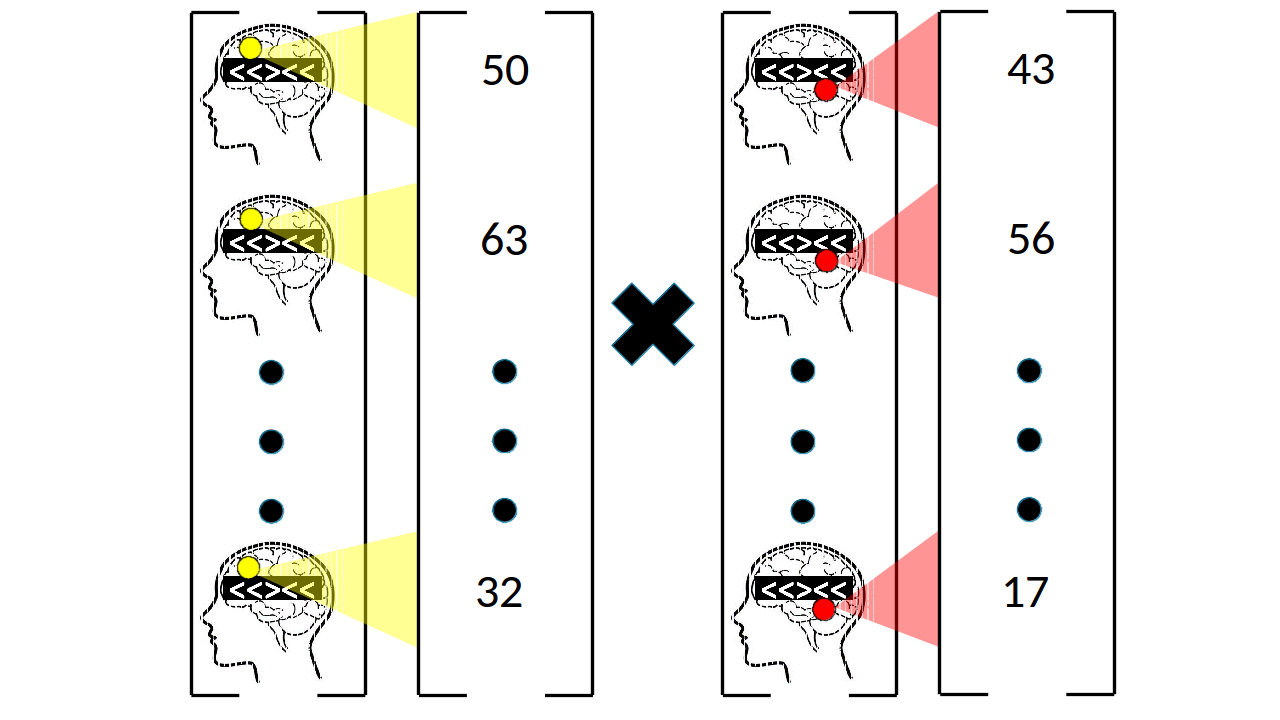
\includegraphics[scale=0.25]{betaseries_correlation_illustration}
    \caption{Setting up beta series Correlations. In the flanker task example above, betas (i.e. activation index) have been fit to every voxel per trial, and separated by condition (incongruent and congruent). This figure is only representing the incongruent trials, but both incongruent and congruent trial data can be collected.Regions of interest (ROIs) can be selected from these beta maps and all the voxels within the ROI are averaged. Once the betas are extracted from each ROI for each trial, the resulting lists of betas can be correlated with each other.}%
    \label{fig:betaseries_correlation_illustration}%    
\end{figure}

The first method is beta series correlations and is sensitive to the theoretical notion of reactive cognitive control (Figure ~\ref{fig:betaseries_correlation_illustration}). 
beta series correlations model the response after a congruent or incongruent stimulus capturing the "on-the-fly" conflict adaptations, otherwise known as reactive cognitive control.
Aim 1 will establish the use of this method due to its novel application to fast-event related designs of fMRI.

The second method is residual correlations; the time-course of the brain's activity after regressing out the stimulus onset information ~\citep{Fair2007,Cole2014,Bolt2017}. 
Residual correlations measure the theoretical notion of proactive cognitive control because proactive cognitive control represents the stable maintenance of goal-relevant task information throughout the performance of the task, which is what the time-series will represent.
Behavioral measures of proactive and reactive cognitive control exist, however outside of the AX-CPT it is difficult to analyze purely proactive and reactive behavioral components. 
Following the characterization of the purported reactive and proactive cognitive control networks, their relationship to existing behavioral measures will be established.
This research will contribute to the ongoing conversation of the neural basis of cognitive control, and provide a more direct metric of these networks during a  cognitive control task.

\section{Specific Aims}
\begin{figure}[H]%
	\centering
	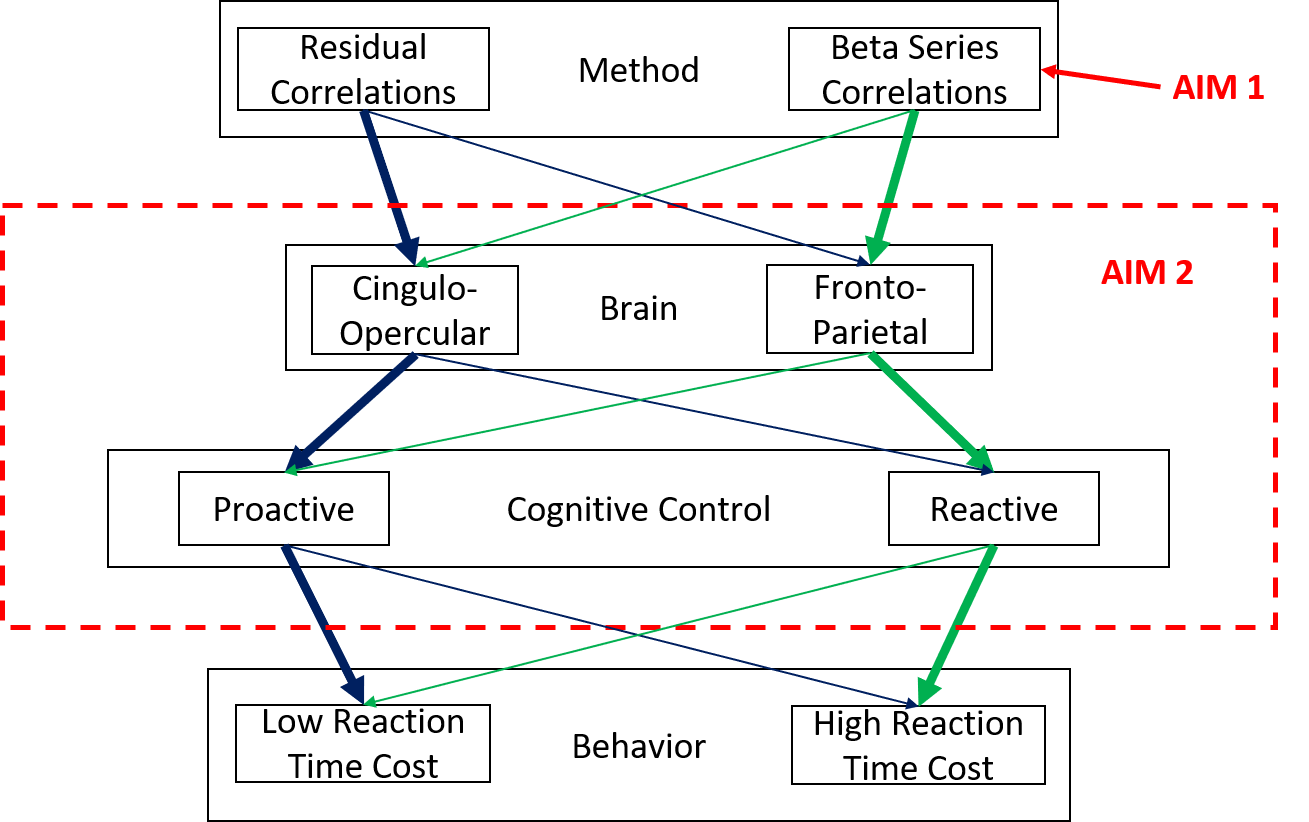
\includegraphics[width=1\linewidth]{overall_thesis_pic}
	\caption{Outline of my three aims. Aim 1 seeks to produce and validate software developed with nipype to perform beta series correlations.
	Aim 2 will profile beta series correlations and residual correlations on the same task datasets to derive differences and similarities between the methods and their relation to reaction time cost}
	\label{fig:all_aims}
\end{figure}

\textbf{Specific Aim 1}: Create and validate NiBetaSeries to perform beta series correlations
\newline
\newline
\textit{Rationale}: A beta in this context refers to the free varying parameter in the general linear model (GLM) that "fits" the data.
\begin{equation}
	Y = X\beta + \epsilon 
	\label{eq:1}
\end{equation}
Equation \ref{eq:1} is the classic GLM where $Y$ represents the time-series we are attempting to explain.
The $\beta$ assumes any value that minimizes the squared error between the modeled data and the actual data. 
$\epsilon$ refers to the error that is not captured by the model.
\begin{equation} \label{eq:2}
Y = X_{Ti}\beta + \epsilon
\end{equation}
Equation \ref{eq:2} describes the least squares separate (LSS) implementation of a GLM, where the major difference is in the design term $X_{Ti}\beta$.
This notation represents that a particular ($Ti$) trial's $\beta$ is being estimated and not the average of all the trials.
Another detail not explicitly noted in the equation is that all other trials of the same type are treated as a single nuisance regressor.
The particular trial's $\beta$ will only account for the unique variance described by that trial.
If there are other trial types, each unique trial type will be its own nuisance regressor containing all trials of that type.
Thus we can account for the unique trial-to-trial variability of the $\beta$s.
\begin{algorithm}
	\caption{Beta Series Algorithm}\label{al:1}
	\begin{algorithmic}[1]
		\FOR{\texttt{Ti in Trials}}
    		\STATE \texttt{$Y = X_{Ti}\beta + \epsilon$}
		\ENDFOR
	\end{algorithmic}
\end{algorithm}
The algorithm to calculate each trial's $\beta$ estimate will be iteratively performed across trials and depending on the trial's condition (e.g. congruent vs. incongruent), the $\beta$ value will be placed in its corresponding list (Algorithm ~\ref{al:1}).
While programs exist to compute beta series correlations, there isn't one that utilizes least squares separate estimation, a modeling strategy that would help with deriving betas from fast event related designs with beta series correlations ~\citep{Mumford2012,Gottlich2015}. 
The proposed software seeks to fill that gap (Figure ~\ref{fig:all_aims}).
\newline
\newline
\textit{Hypothesis}:
The beta series software will capture brain response variability across trials to produce correlations that are different from resting state correlations.
\newline
\newline
\textit{Method}:
Under the Nipype framework, I will use python to model data on a trial-by-trial basis ~\citep{Smith2004,Gorgolewski2017}. 
Using a traditional GLM with a double gamma basis function, modeling will be completed by performing a GLM for each trial individually, with all other trials of the same type combined into a single term to form a regressor of non-interest ~\citep{Mumford2012}.
Additionally, trials from other trial types will each get their own regressor.

Validation of the beta series software will be shown in three steps progressively from simulations to real data.
The first question I'm answering is \textbf{whether NiBetaSeries is able to capture BOLD response correlations.}
Starting from simulations, two voxels will be simulated with a specified correlation of BOLD responses that I control.
I will vary the correlation between the two voxels and inject different amounts of noise to ascertain how well nibetaseries recaptures the correlation I set between the two voxels.
From these simulations I will be able to approximate power for subsequent analyses.

\begin{figure}[H]%
	\centering
	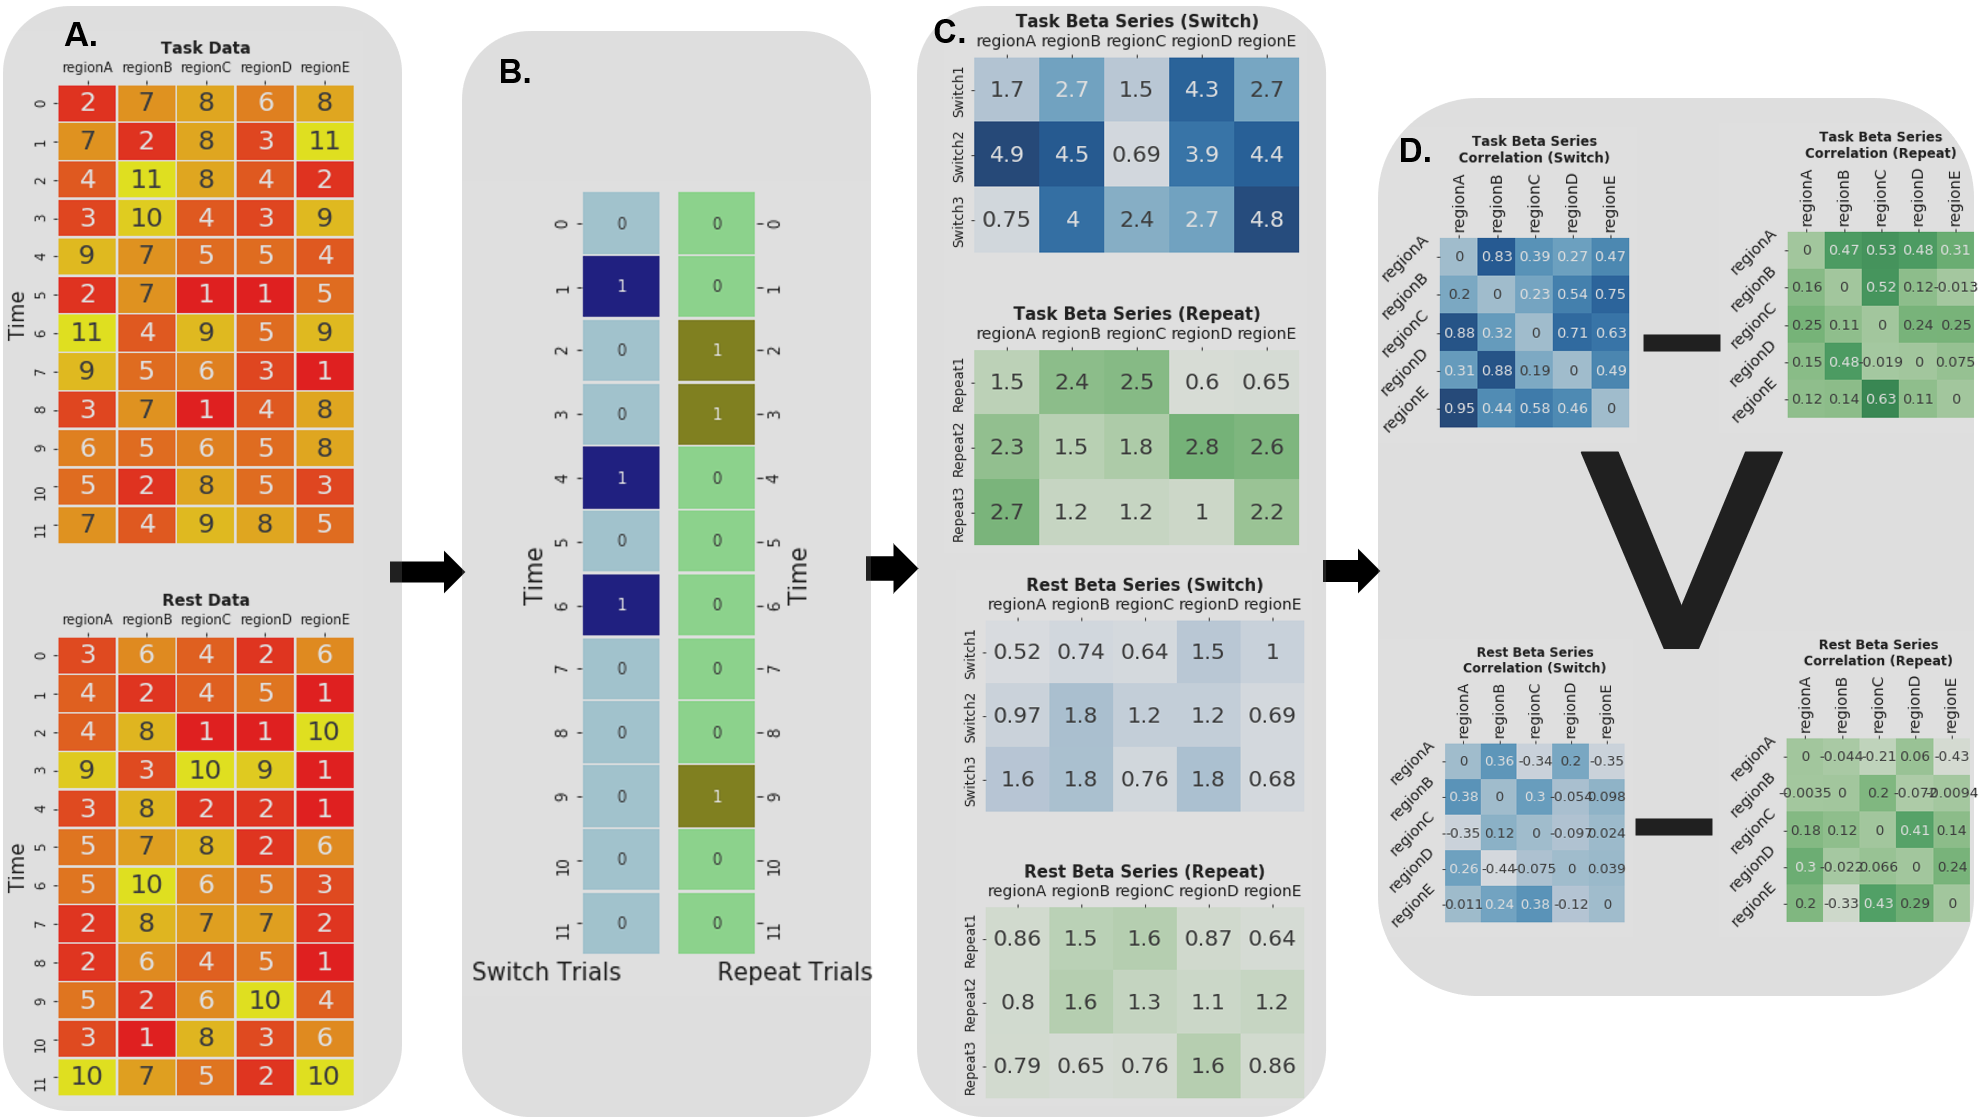
\includegraphics[width=1\linewidth]{validation_of_beta_series_pt_1}
	\caption{Applying Beta Series to both task and rest BOLD data.
	A) Flattened example task and resting state BOLD data are illustrated with 5 regions/voxels and 12 time points.
	Resting state data is being treated as if a task was performed.
	B) The two trial types in the task: switch and repeat. While the events did not actually occur during the resting state scan,
	I am treating the resting state data as though the events did occur.
	C) The expected betas series for the task and rest data.
	Note in the task data the switch trial type has higher betas on average relative to the repeat trial type.
	The trial types in the rest data should have similar betas since there was no actual task performed.
	D) The beta series are correlated between all regions for all trial types resulting in four 5x5 matrices.
	I expect the difference between the switch and repeat trial types in the task data to be greater than
	the difference between the switch and repeat trial types in the rest data.}
	\label{fig:validation_of_beta_series_pt_1}
\end{figure}

The second question I'm answering is \textbf{whether beta series correlations rely on the BOLD response to detect task-modulated differences}. 
The second validation will proceed by comparing task data with resting state data (Figure ~\ref{fig:validation_of_beta_series_pt_1}).
The resting state data will be analytically treated the same as the task data, testing the assertion nibetaseries uses the BOLD response to capture correlations between brain regions.
Brain regions and networks will be defined with the Schaefer 400 atlas ~\citep{schaefer2017}.
Beta series correlation matrices will be derived for repeat and switch trials separately for both task and rest resulting in four correlation matrices.
Beta series correlations will be averaged within the Schaefer control network, compressing the data to four observations per participant.
A linear mixed effects model will be run to test if the difference between switch and repeat can only be seen with the task beta series correlations.
The average correlation will be the dependent measure; data type (i.e., task or rest) and trial type (i.e., switch or repeat) will be the categorical predictors; and participant will have a random intercept.
I hypothesize there will be a significant interaction between data type and trial type where the difference between switch and repeat is greater for task beta series correlations relative to the rest beta series correlations.

\begin{figure}[H]%
	\centering
	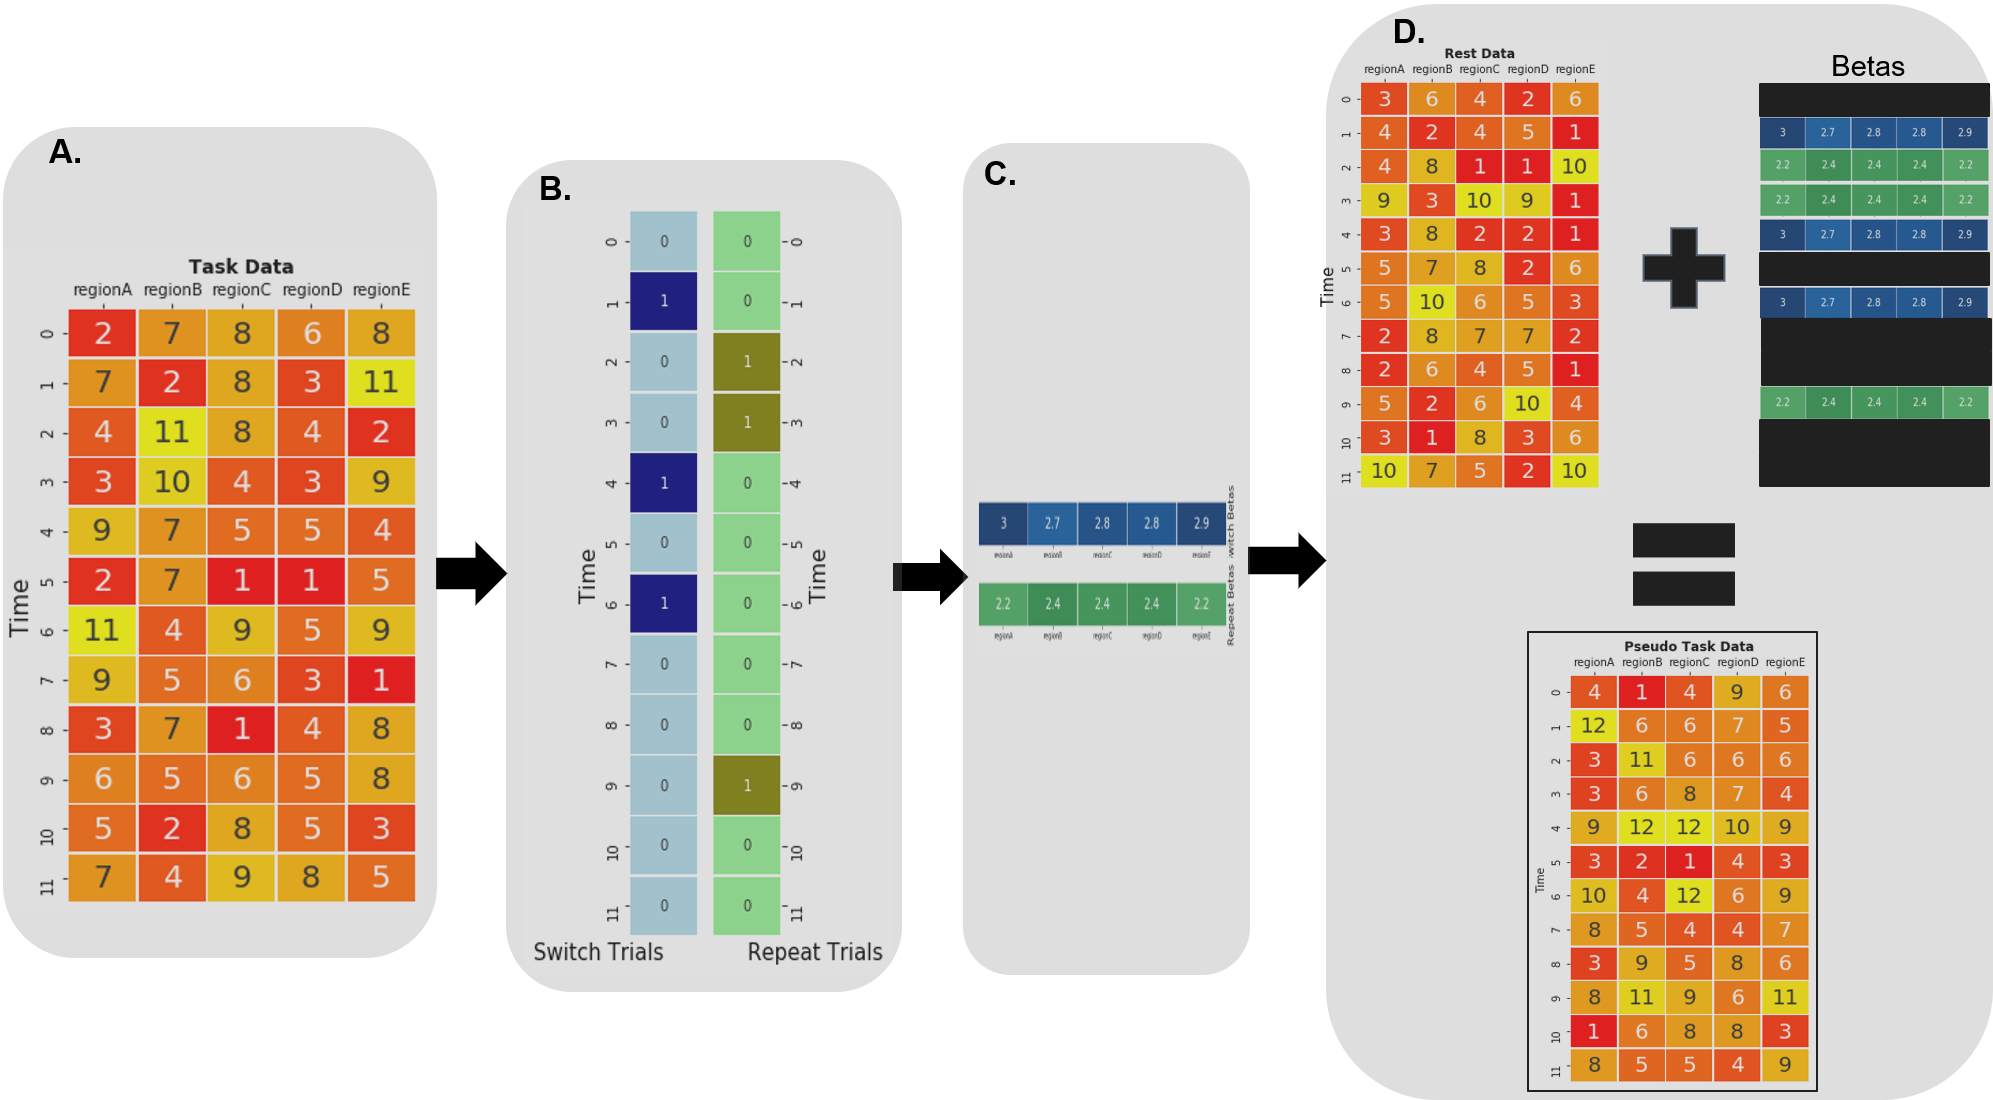
\includegraphics[width=1\linewidth]{validation_of_beta_series_pt_2}
	\caption{Creating Pseudo Task data from resting state data.
	A) Starting with the example flattened task BOLD data, B) calculate the average response of the task BOLD data
	to the two trial types (Switch and Repeat).
	C) Once the average responses (or betas) are calculated,
	D) I will take the resting state data and add the average responses back into the task BOLD data
	every time that trial type occurs.
	With the "pseudo-task" BOLD data, I can treat it as I would normal task BOLD data and calculate beta series
	correlations.
	}
	\label{fig:validation_of_beta_series_pt_2}
\end{figure}

The third question I'm answering is \textbf{if beta series correlations are driven by ongoing resting state fluctuations or by BOLD response variability dependent on task demands.}
BOLD response variability could merely be a reflection of ongoing resting state fluctuations and not a representation of brain reconfiguration driven by task demands (e.g., such as whether the trial type is switch or repeat).
If BOLD response variability is driven by resting state fluctuations, the difference in correlations between the switch and repeat trials would be attributable to the differences in response magnitude for each trial type.
In other words, the larger the BOLD response, the easier it is to detect the ongoing resting state correlations.
The third and final validation will be identical to the previous analysis, except the resting state data will have inserted task evoked responses creating “pseudo-task” data (Figure ~\ref{fig:validation_of_beta_series_pt_2}).
The resting state data will be convolved with a hemodynamic response that represents the average response for each unique trial type for a participant.
For every trial, the corresponding hemodynamic response for that trial type will be fit to every voxel.
If engaging in a task only adds BOLD responses to the ongoing resting state activity, the correlation matrices from the “pseudo-task” data and the task data should be close to each other.
However, if there is variance in the BOLD response that is independent of the ongoing resting state activity, the correlation matrices from the “pseudo-task” data and the task data should be different.
This test may provide evidence that beta series correlations capture unique variance not explained by resting state fluctuations, validating the utility of beta series correlations to answer novel questions about brain activity during a task.
\begin{figure}[H]%
	\centering
	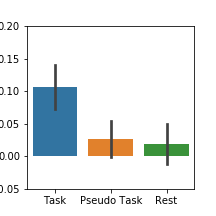
\includegraphics[width=1\linewidth]{aim_1_validation}
	\caption{Expected results from the real data validation.
	I expect the difference in beta series correlations between switch and repeat trial types should be the largest in the real task BOLD data and significantly greater than "pseudo-task" BOLD data and resting state BOLD data}
	\label{fig:aim_1_validation}
\end{figure}
The pattern of hypothesized trial-type differences for task, "pseudo-task" and rest is seen in Figure ~\ref{fig:aim_1_validation}.
\newline
\newline
\textit{Alternative Methods}: If the beta series approach introduces bias into the correlation measures (e.g., all regions are strongly correlated with each other), the method to derive betas will be re-evaluated.
If there is not a suitable method to reduce/remove the bias, psycho-physiological interactions (PPI) may be used instead to derive relative trial activation, although there is no a priori reason to believe PPI will be less susceptible to bias.
If averaging correlations within a network does not capture the data type by trial type interaction, multivariate methods may be used.
Specifically, a classifier could be trained on the correlation matrices to identify each of the categories (e.g., rest-switch, rest-repeat, task-switch, task-repeat)
leveraging the full correlation matrix.
Another option is to use graph theoretical measurements such as local or global efficiency to capture the state of overall network.
\newline
\newline
\textbf{Specific Aim 2}: Characterize the relationship between beta series correlations (reactive) and residual correlations (proactive) during a flanker task.
\newline
\newline
\textit{Rationale}: The dual mechanisms of control theory posits these networks should be differentially sensitive to the type of correlation method applied ~\citep{Dosenbach2007,Braver2006}.
However, work by Michael Cole suggests there will not be large differences between residual correlations and beta series correlations ~\citep{Cole2019}.
Despite the suggestion by Michael Cole's work, the differences between residual correlations and beta series correlations have not been explicitly tested.
This gap presenting an excellent opportunity to conceptually frame task data into stimulus evoked components and persistent residual components.
\newline
\newline
\textit{Hypothesis}:
I hypothesize the cingulo-opercular network will be modulated by proactive cognitive control and will be detectable with residual time series, but not beta series.
My complementary hypothesis states the frontal-parietal network will be modulated by reactive cognitive control and will be detectable with beta series, but not residual time series. 
\newline
\newline
\textit{Methods}:
Data from the openneuro dataset \href{https://openneuro.org/datasets/ds001751/versions/1.0.0}{ds001751} will be used to measure both beta series and residual correlations during a Flanker task.
The task has two block types, mostly incongruent (80 percent incongruent) and mostly congruent (20 percent incongruent).
The mostly incongruent block incites proactive cognitive control because the participant is likely to have to resolve a stimulus conflict for each trial.
On the other hand, the mostly congruent block encourages reactive control because the participant is not likely to see a conflicting stimulus.
All participants went through both congruent and incongruent blocks constituting a fully within subjects design.
The behavioral results indicate a successful manipulation of the congruency effect ~\citep{Aben2019}.
The participants had a much smaller congruency effect (measured with reaction time series) during the mostly incongruent block relative to the mostly congruent block.
For each participant, I will be able to measure both beta series correlations and residual correlations during mostly incongruent blocks and mostly congruent blocks. 
Using the Dosenbach ROIs, I will create correlation matrices for both beta series and residual time series ~\citep{Dosenbach2010}.
I will test the robustness of the results using the Schaefer atlas as an alternative atlas ~\citep{schaefer2017}.

\begin{figure}[H]%
	\centering
	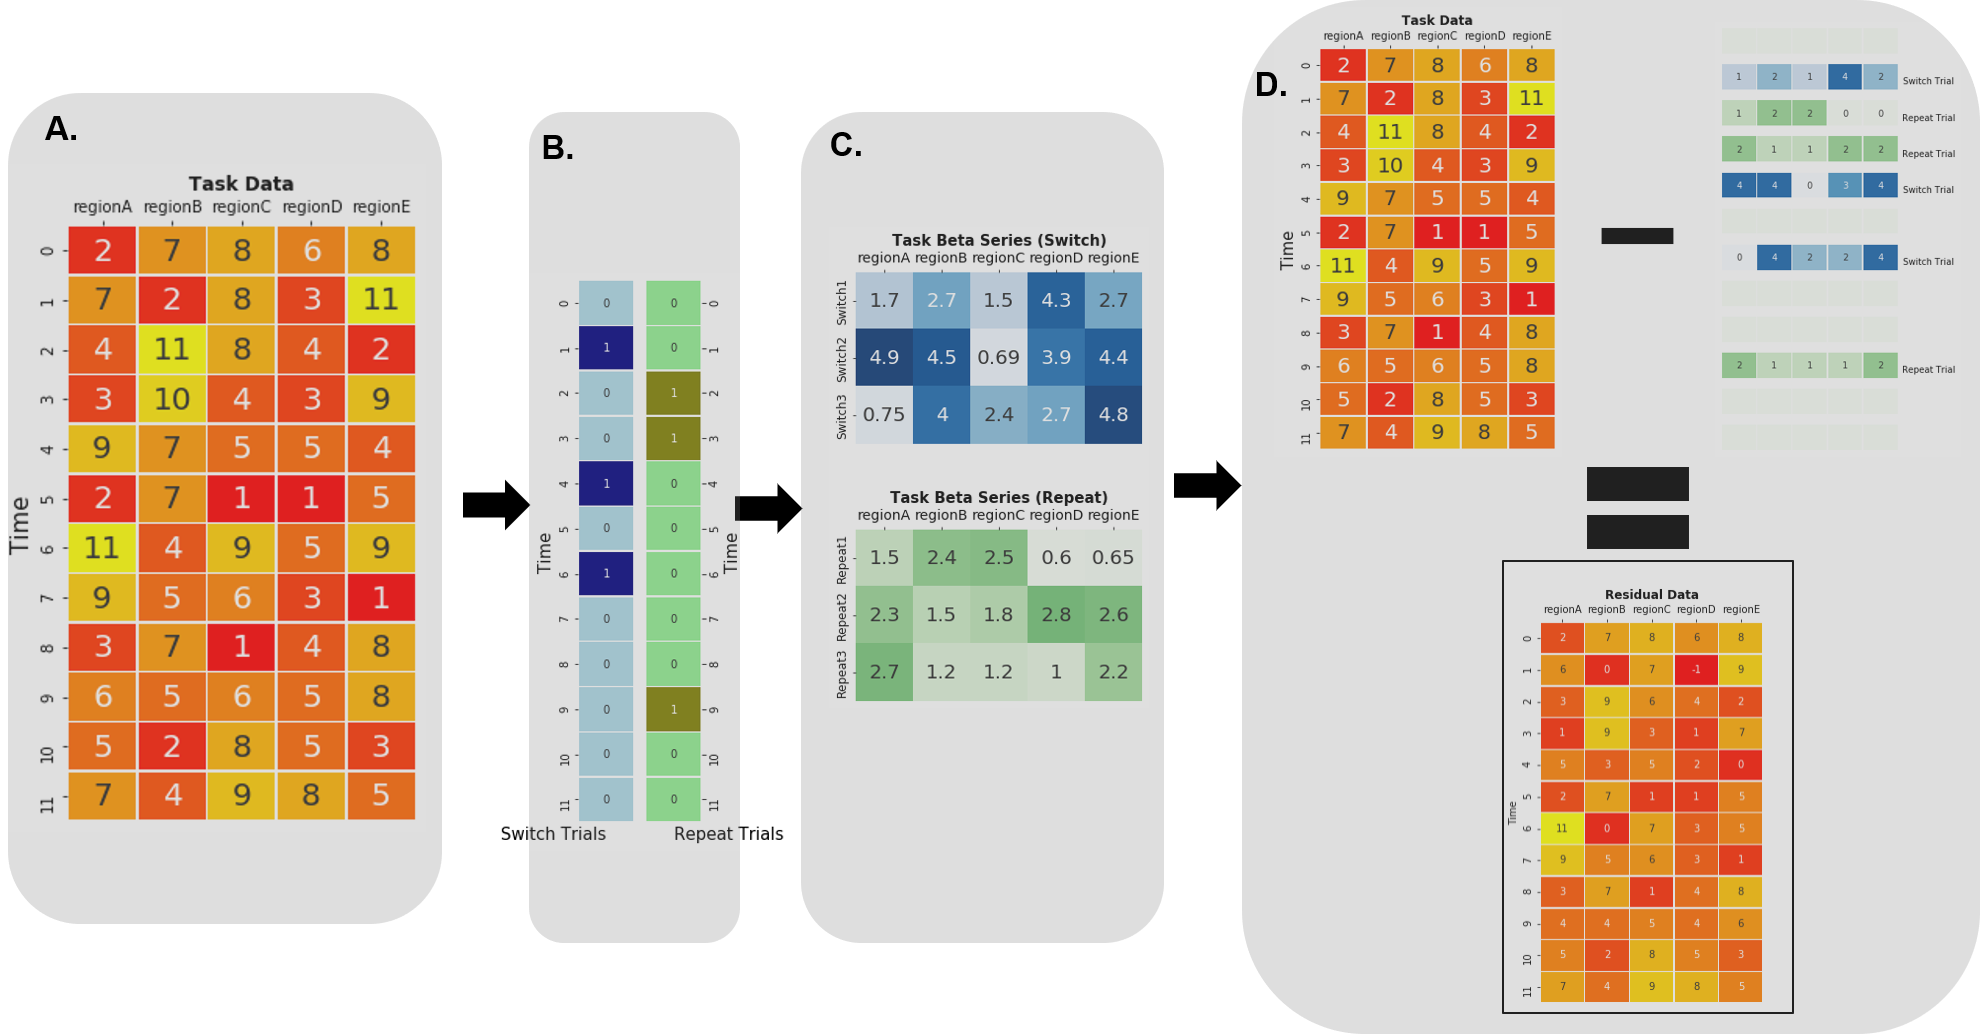
\includegraphics[width=1\linewidth]{residual_correlations}
	\caption{Calculating Residual Correlations.
	A) Flattened and simplified task BOLD data with 12 time points and 5 regions/voxels.
	B) Each trial onset will get its own regressor in a GLM to
	C) calculate an individual beta per trial, resulting in a beta series.
	D) The beta series will be subtracted from the original task BOLD data, removing potential
	trial modulated BOLD response variance, only leaving the variance attributed to task context (e.g., whether the block was congruent or incongruent).}
	\label{fig:residual_correlations}
\end{figure}

To calculate residual correlations four steps will be completed ~\ref{fig:residual_correlations}.
First, the stimulus responses will be modeled and removed from the data.
To remove the stimulus responses, stimulus onsets from the task will be represented as impulses and convolved with a double gamma as the basis function for the GLM. 
Each stimulus event will entered into the GLM as its own regressor.
This ensures the trial-to-trial variance will be removed from the task data, and not just the mean response of a stimulus. 
The residual data from the GLM will represent BOLD responses not captured by direct responses to stimuli. 
Second, the data will be split into the mostly congruent block and mostly incongruent blocks.
The splitting allows me to analyze the state dependent correlations during the mostly congruent and mostly incongruent blocks separately.
Third, the data will be z-transformed to normalize the distributions and Pearson's R correlations will be extracted from ROIs that participate in the fronto-parietal network and the cingulo-opercular network.
Fourth, ROIs that belong to the same network will be correlated with each other and averaged giving an average within network correlation.

Beta series will be calculated as described in aim 1.
The correlations will be performed similarly to the residual correlations, except instead of residuals, the beta maps will be normalized and within network correlations will be calculated for the incongruent trial type within the mostly incongruent and mostly congruent blocks.
Average within network correlations for the cingulo-opercular and fronto-parietal networks across participants for both beta series and residual correlations in the mostly incongruent block and mostly congruent block serve as the primary outcome measure.
I will look at change in within network correlations as a function of the network (fronto-parietal and cingulo-opercular) by block (mostly incongruent and mostly congruent) by method (residual and beta series correlations) using mixed effects modeling with a random intercept for participant.
I predict a significant network by block by method interaction ~\ref{fig:aim_2_validation}.
\begin{figure}[H]%
	\centering
	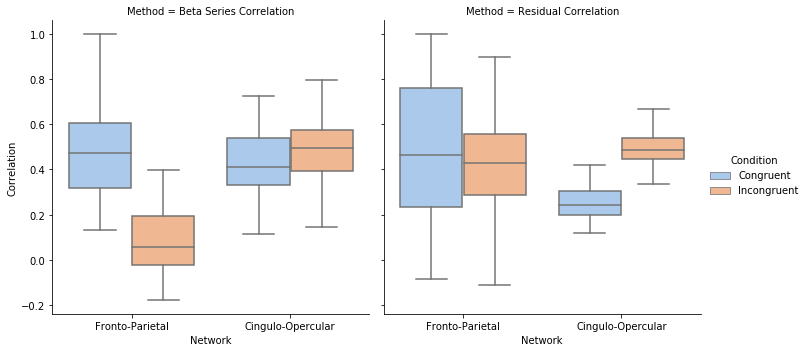
\includegraphics[width=1\linewidth]{aim_2_validation}
	\caption{Hypothesized relationship between network (fronto-parietal and cingulo-opercular), method (beta series and residual), and block (mostly congruent and mostly incongruent).
	I hypothesize the fronto-parietal network beta series correlation should be lower during the incongruent block relative to the congruent block.
	There is not a strong prediction on how the cingulo opercular network will behave with beta series correlations.
	I also hypothesize the cingulo-opercular network residual correlation should be higher during the incongruent block relative to the congruent block.
	There is not a strong prediction on how the fronto-parietal network will behave with residual correlations.}
	\label{fig:aim_2_validation}
\end{figure}
From this interaction I expect the within network residual correlations from the cingulo-opercular network to increase during the mostly incongruent block relative to the mostly congruent block.
This prediction supports the proactive role of the cingulo-opercular network which is proposed to be online during the entirety of the mostly incongruent block.
I also expect the within network beta series correlations from the fronto-parietal network to increase during the mostly congruent block relative to the mostly incongruent block.
This prediction supports the reactive role of the fronto-parietal network which is only called upon during the incongruent trials within the mostly incongruent block.
\newline
\newline
\textit{Alternative Methods}:
Beta series correlations give correlations for each trial type (incongruent and congruent), but in the proposed methods I only anticipate the incongruent trials to have explanatory power.
However, it could be the relationship between congruent and incongruent trial types changes between the blocks suggesting subtracting the congruent correlation matrix from the incongruent correlation matrix would be more sensitive to the difference between blocks.
The mixed effects regression may also contain quality metrics of the data including average framewise displacement and global correlation to rule out noise driving the observed effect. 
If within network correlations from mixed effects regression do not adequately model the differences, I can use graph theoretical measures such as participation coefficient and efficiency.
\newline

%=============================================================================
\chapter{NiBetaSeries}
%=============================================================================

Beta series correlations appeared exciting when initially produced ~\citep{Rissman2004},
but have been relegated to post-hoc analyses being used as almost an afterthought in many
publications (add citations).
There was a brief resurgence when Benjamin Turner, Jeannette Mumford, and Hunar Abdulrahman... repurposed
beta series for classification of different trial types; however beta series correlations
remained under used.
Beta series correlations give a lens into how the brain's organization changes depending
on cognitive state, the theoretical implications would be fruitful for the field of neuroscience.
Then why aren't more researchers looking at beta series correlations?
Surveying the existing toolboxes available for calculating beta series correlations reveals a
potential answer.
A couple toolboxes that calculate beta series include BASCO, pybetaseries, and pyMVPA.
However, BASCO has limitations on the number of methods you can use to generate beta series,
pybetaseries is no longer being actively developed, and pyMVPA requires the user to know
a decent amount of python to make use of their functions.
With the limitations of the current toolboxes and the relative anonymity of beta series,
it comes with little surprise that many researchers do not use this method and instead reach for
more familiar analyses using General Linear Models (GLMs) or resting state correlations applied
to task data (add citation).

To change this trend and make beta series more accessible, I've created a toolbox called NiBetaSeries.
NiBetaSeries leverages the latest trends in the python neuroimaging world and adds to the flourishing
ecosystem of tools that share a core organizational philosophy.
This tool calculates betaseries correlations for the user and passes the beta series images themselves
for the user to decide what analysis method they wish to pursue.

With the creation of this toolbox, I can test another reason for the dearth of published materials on
beta series correlations.
Namely, most researchers may not have found any results with beta series correlations.
In this chapter; I will explore under what experimental conditions NiBetaSeries is useful and offer
recommendations for when to use the toolbox.

\section{Simulations}
Simulation in fMRI has a rich literature, with multiple strategies varying along the axis
of practicality and accuracy.
For testing tools/methods on many different experimental designs; simulating the bloch equations
is too computationally intensive and simpler simulations can generate realistic data.
To this author's knowledge, the first accessible tool to generate simulated fMRI data is NeuRoSim (add citation).
NeuRoSim allows the user to create expected responses to stimuli, motion noise, physiological noise,
time series drift, and autocorrelation of the time series (add citation).
More recently, the python module fmrisim was released mirroring the functionality of NeuRoSim, making this tool
the ideal choice to test NiBetaSeries; another python application.


\section{Real Data}

%=============================================================================
\chapter{Residual Correlations}
%=============================================================================
Talk all about Micheal Cole...

%=============================================================================
\chapter{Beta Series versus Residual Correlations}
%=============================================================================

\section{Residual Correlations}


%=============================================================================
\chapter{General Discussion}
%=============================================================================

%=============================================================================
\appendix
%=============================================================================

%=============================================================================
\chapter{Sample Appendix}

\section{Appendix One}
\blindtext

\section{Appendix Two}
\blindtext

%=============================================================================
\chapter{Another Appendix}

\section{Appendix Three}
\blindtext


%=============================================================================
% bibliography
%=============================================================================
\interlinepenalty=10000	% prevents bib items from splitting across pages
\bibliographystyle{uithesis}
\bibliography{thesis} 

\end{document}

% Thesis Comments
% compare relative to PPI
% split the results into two methods, here's my added value
% add on participants for correlations to lss/lsa
% beta versus PPI (AIM 2)
% why we care about connectivity,
% and why we care about task related connectivity
% 
Meeting Notes
Discussion to change Aim's 1 and 2 for the pragmatic purpose
of getting a paper submitted.
Change Aim1:
split dataset into two halves (compare LSS and LSA)
Change Aim2:
split dataset into two halves (compare LSS and PPI)